\section{Construction and first properties}

In this section, after recalling some notations, the partial order
$\Dyck_n$ is defined through its Hasse diagram. Some properties of
this partial order are proved.

\label{sec1}
A \defin{Dyck path} of size $n \geq 0$ is a lattice path from $(0,0)$ to
$(2 n,0)$ using only north-east and south-east steps and staying weakly above
the horizontal line.

We will also consider Dyck paths of size $n$ as words of length $2 n$
in the alphabet $\{0,1\}$, where $1$ stands for a north-east step and
$0$ for a south-east step.

\begin{figure}[htb]\centering
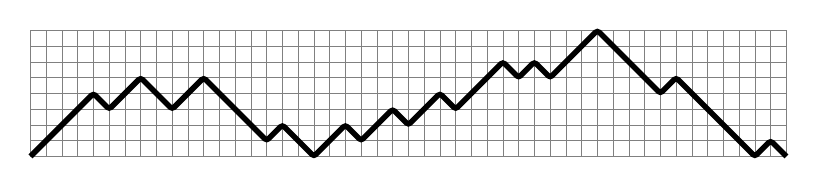
\begin{tikzpicture}[scale=0.2]
\draw[gray,very thin] (0, 0) grid (48, 8);  
\draw[rounded corners=1, color=black, line width=2] (0, 0) -- (1, 1) -- (2, 2) -- (3, 3) -- (4, 4) -- (5, 3) -- (6, 4) -- (7, 5) -- (8, 4) -- (9, 3) -- (10, 4) -- (11, 5) -- (12, 4) -- (13, 3) -- (14, 2) -- (15, 1) -- (16, 2) -- (17, 1) -- (18, 0) -- (19, 1) -- (20, 2) -- (21, 1) -- (22, 2) -- (23, 3) -- (24, 2) -- (25, 3) -- (26, 4) -- (27, 3) -- (28, 4) -- (29, 5) -- (30, 6) -- (31, 5) -- (32, 6) -- (33, 5) -- (34, 6) -- (35, 7) -- (36, 8) -- (37, 7) -- (38, 6) -- (39, 5) -- (40, 4) -- (41, 5) -- (42, 4) -- (43, 3) -- (44, 2) -- (45, 1) -- (46, 0) -- (47, 1) -- (48, 0);
\end{tikzpicture}
\caption{A typical example}
\label{typique}
\end{figure}
\Cref{typique} displays a typical example.

The \defin{area} under a Dyck path is the surface of the domain between
the horizontal line and the Dyck path.

Every Dyck path can be uniquely written as the concatenation of
several blocks, where in every block the only vertices on the
horizontal line are the first and last ones. If there is only one
block, the Dyck path is said to be \defin{block-indecomposable}. The
example displayed above has $3$ blocks.

Inside a Dyck path, a subsequence of consecutive steps is called a
\defin{subpath} if it starts and ends at the same height and keeps
strictly above that height in between. Here the height is the
vertical coordinate, increased by north-east steps and decreased by
south-east steps.

Let us say that a subpath $x$ of a Dyck path $w$ is \defin{movable} if
it is preceded in $w$ by the letter $0$ and
\begin{itemize}
\item either $x$ ends at the last letter of $w$,
\item or $x$ is followed in $w$ by the letter $1$.
\end{itemize}

\begin{figure}[htb]\centering
\begin{minipage}[b]{0.5\textwidth}\centering
\begin{tikzpicture}[scale=0.35]
  \draw[gray,very thin] (0, 0) grid (10, 2);
  \draw[rounded corners=1, color=black, line width=2] (0, 0) -- (1, 1) -- (2, 0) -- (3, 1) -- (4, 2) -- (5, 1) -- (6, 2) -- (7, 1) -- (8, 0) -- (9, 1) -- (10, 0);
  \draw[rounded corners=1, pattern=north west lines, pattern color=teal] (5, 1) -- (6, 2)-- (7, 1) ;
\end{tikzpicture}
\caption{A subpath which is not movable.}\end{minipage}\hfill
\begin{minipage}[b]{0.45\textwidth}\centering
\begin{tikzpicture}[scale=0.35]
  \draw[gray,very thin] (0, 0) grid (10, 2);
  \draw[rounded corners=1, color=black, line width=2] (0, 0) -- (1, 1) -- (2, 0) -- (3, 1) -- (4, 2) -- (5, 1) -- (6, 2) -- (7, 1) -- (8, 0) -- (9, 1) -- (10, 0);
  \draw[rounded corners=1, pattern=north west lines, pattern color=teal] (2, 0) -- (3, 1) -- (4, 2) -- (5, 1) -- (6, 2) -- (7, 1) -- (8, 0);
\end{tikzpicture}\caption{A movable subpath.}\end{minipage}\hfill

\vspace*{5mm}
\begin{minipage}[b]{0.45\textwidth}\centering
\begin{tikzpicture}[scale=0.35]
  \draw[gray,very thin] (0, 0) grid (10, 2);
  \draw[rounded corners=1, color=black, line width=2] (0, 0) -- (1, 1) -- (2, 0) -- (3, 1) -- (4, 2) -- (5, 1) -- (6, 2) -- (7, 1) -- (8, 0) -- (9, 1) -- (10, 0);
  \draw[rounded corners=1, pattern=north west lines, pattern color=teal] (8, 0) -- (9, 1) -- (10, 0);
\end{tikzpicture}\caption{A movable subpath.}\end{minipage}
\end{figure}

For every Dyck path $w$ and every movable subpath $x$ in $w$, let
$N(w,x)$ be the number of consecutive $0$ letters that appear just
before $x$. For any integer $1 \leq i \leq N(w,x)$ (corresponding to a
choice among the consecutive $0$ letters just before $x$), let us
define another Dyck path $M(w,x,i)$ as the following word:
\begin{itemize}
\item first the initial part of $w$ until the letter before the chosen $0$,
\item then $x$,
\item then the $0$ letters starting at the chosen $0$,
\item then the final part of $w$ after $x$.
\end{itemize}
Graphically, this transformation corresponds to sliding the
subpath $x$ in the north-west direction by one or several steps.

%

\begin{figure}[htb]\centering
\begin{tikzpicture}[scale=0.4]  
\draw[gray,very thin] (0, 0) grid (12, 3);  
\draw[rounded corners=1, color=black, line width=2] (0, 0) -- (1, 1) -- (2, 2) -- (3, 3) -- (4, 2) -- (5, 3) -- (6, 2) -- (7, 1) -- (8, 0) -- (9, 1) -- (10, 2) -- (11, 1) -- (12, 0);
\draw[rounded corners=1, pattern=north west lines, pattern color=teal] 
(8, 0) -- (9, 1) -- (10, 2) -- (11, 1) -- (12, 0);
\end{tikzpicture}\hfill\put(35,15){$\longrightarrow$}\hfill%
\begin{tikzpicture}[scale=0.4]  
\draw[gray,very thin] (0, 0) grid (12, 4);  
\draw[rounded corners=1, color=black, line width=2] (0, 0) -- (1, 1) -- (2, 2) -- (3, 3) -- (4, 2) -- (5, 3) -- (6, 2) -- (7, 3) -- (8, 4) -- (9, 3) -- (10, 2) -- (11, 1) -- (12, 0);
\draw[rounded corners=1, pattern=north west lines, pattern color=teal] 
(6, 2) -- (7, 3) -- (8, 4)-- (9, 3) -- (10, 2);
\end{tikzpicture}
\caption{A cover relation $w \to w'$}
\end{figure}


Let $\Dyck_n$ be the set of Dyck paths of size $n$. Let us
introduce a directed graph $\Gamma_n$ with vertex set $\Dyck_n$. It
has edges from every Dyck path $w$ to all Dyck paths $M(w,x,i)$ where
$x$ is a movable subpath of $w$ and $i$ an integer between $1$ and
$N(w,x)$.

Let $\wmin$ be the unique Dyck path made of
alternating $1$ and $0$.
\begin{prop}
  The directed graph $\Gamma_n$ is connected and acyclic with $\wmin$ as
  unique source element.
\end{prop}
\begin{proof}
  First, every edge in $\Gamma_n$ increases strictly the area under
  the Dyck path, so there cannot be any oriented cycles.

  Let $w$ be any Dyck path not equal to $\wmin$. Then $w$ has at
  least one block $x$ of maximal height at least $2$. This block ends by a
  sequence of at least two $0$ preceded by a $1$. Let $w'$ be the Dyck
  path obtained by exchanging this $1$ and that sequence of $0$ except
  the last one. Then there is an edge in $\Gamma_n$ from $w'$ to $w$.

  Therefore, $\wmin$ is the unique source element in
  $\Gamma_n$. Together with the absence of oriented cycles, this
  implies that for every Dyck path $w$, there exists a path in
  $\Gamma_n$ from $\wmin$ to $w$.
\end{proof}

\begin{prop}
  The directed graph $\Gamma_n$ is the Hasse diagram of a partial order.
\end{prop}
\begin{proof}
  This means that $\Gamma_n$ is acyclic and transitively reduced. It
  remains only to prove the second property.
  
  So let us consider an edge $w \to M(w,x,i)$ and assume that one can
  find a sequence~(S) of edges $w \to M(w,x',i') \to \dots \to M(w,x,i)$.

  Every edge in $\Gamma_n$ can be considered as a sequence of several
  moves where a subpath is slid by just one step in the north-west
  direction. As recalled in Appendix A, these sliding moves are
  exactly the cover relations in the Tamari partial order on the same
  set of Dyck paths.

  Therefore, one can refine the sequence (S) of edges in $\Gamma_n$
  into a sequence of cover relations in the Tamari lattice. By
  Lemma A.1, the interval in the Tamari lattice between $w$
  and $M(w,x,i)$ is just a chain obtained by repeated sliding of the subpath~$x$. 
  This implies that all the intermediate vertices of the
  sequence (S) are obtained by sliding the same subpath $x$.

  But in the graph $\Gamma_n$, there cannot be any two consecutive
  edges where exactly the same subpath is slid. Indeed, after being
  slid once, the subpath is followed by a letter~$0$, hence no
  longer movable. It follows that the sequence (S) is reduced to the
  single edge $w \to M(w,x,i)$.
\end{proof}


Let us denote by $\sm$ the partial order relation on $\Dyck_n$ thus defined. The edges of $\Gamma_n$ are now understood as the cover relations in the poset $(\Dyck_n, \sm)$.

\medskip

We propose to call this partial order the \defin{dexter order} on Dyck
paths. This choice of terminology is motivated by the fact that the
cover relations are shortcuts (dexterity) and that a symmetry is
broken when compared to the Tamari lattice (dexter in the context of
chirality).

\begin{figure}[htb]
  \centering
  \begin{tikzpicture}[>=latex,line join=bevel,scale=0.3]
%
\node (node_2) at (876.0bp,107.0bp) [draw,draw=none] {$\vcenter{\hbox{$\begin{tikzpicture}[scale=0.15]  \draw[gray,very thin] (0, 0) grid (8, 2);  \draw[rounded corners=1, color=black, line width=1.5] (0, 0) -- (1, 1) -- (2, 0) -- (3, 1) -- (4, 2) -- (5, 1) -- (6, 0) -- (7, 1) -- (8, 0);\end{tikzpicture}$}}$};
  \node (node_3) at (1129.0bp,223.0bp) [draw,draw=none] {$\vcenter{\hbox{$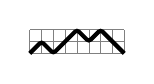
\begin{tikzpicture}[scale=0.15]  \draw[gray,very thin] (0, 0) grid (8, 2);  \draw[rounded corners=1, color=black, line width=1.5] (0, 0) -- (1, 1) -- (2, 0) -- (3, 1) -- (4, 2) -- (5, 1) -- (6, 2) -- (7, 1) -- (8, 0);\end{tikzpicture}$}}$};
  \node (node_9) at (370.0bp,367.0bp) [draw,draw=none] {$\vcenter{\hbox{$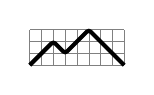
\begin{tikzpicture}[scale=0.15]  \draw[gray,very thin] (0, 0) grid (8, 3);  \draw[rounded corners=1, color=black, line width=1.5] (0, 0) -- (1, 1) -- (2, 2) -- (3, 1) -- (4, 2) -- (5, 3) -- (6, 2) -- (7, 1) -- (8, 0);\end{tikzpicture}$}}$};
  \node (node_8) at (117.0bp,367.0bp) [draw,draw=none] {$\vcenter{\hbox{$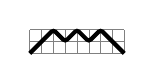
\begin{tikzpicture}[scale=0.15]  \draw[gray,very thin] (0, 0) grid (8, 2);  \draw[rounded corners=1, color=black, line width=1.5] (0, 0) -- (1, 1) -- (2, 2) -- (3, 1) -- (4, 2) -- (5, 1) -- (6, 2) -- (7, 1) -- (8, 0);\end{tikzpicture}$}}$};
  \node (node_7) at (117.0bp,223.0bp) [draw,draw=none] {$\vcenter{\hbox{$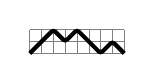
\begin{tikzpicture}[scale=0.15]  \draw[gray,very thin] (0, 0) grid (8, 2);  \draw[rounded corners=1, color=black, line width=1.5] (0, 0) -- (1, 1) -- (2, 2) -- (3, 1) -- (4, 2) -- (5, 1) -- (6, 0) -- (7, 1) -- (8, 0);\end{tikzpicture}$}}$};
  \node (node_6) at (370.0bp,223.0bp) [draw,draw=none] {$\vcenter{\hbox{$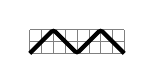
\begin{tikzpicture}[scale=0.15]  \draw[gray,very thin] (0, 0) grid (8, 2);  \draw[rounded corners=1, color=black, line width=1.5] (0, 0) -- (1, 1) -- (2, 2) -- (3, 1) -- (4, 0) -- (5, 1) -- (6, 2) -- (7, 1) -- (8, 0);\end{tikzpicture}$}}$};
  \node (node_5) at (370.0bp,107.0bp) [draw,draw=none] {$\vcenter{\hbox{$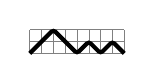
\begin{tikzpicture}[scale=0.15]  \draw[gray,very thin] (0, 0) grid (8, 2);  \draw[rounded corners=1, color=black, line width=1.5] (0, 0) -- (1, 1) -- (2, 2) -- (3, 1) -- (4, 0) -- (5, 1) -- (6, 0) -- (7, 1) -- (8, 0);\end{tikzpicture}$}}$};
  \node (node_4) at (623.0bp,223.0bp) [draw,draw=none] {$\vcenter{\hbox{$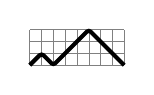
\begin{tikzpicture}[scale=0.15]  \draw[gray,very thin] (0, 0) grid (8, 3);  \draw[rounded corners=1, color=black, line width=1.5] (0, 0) -- (1, 1) -- (2, 0) -- (3, 1) -- (4, 2) -- (5, 3) -- (6, 2) -- (7, 1) -- (8, 0);\end{tikzpicture}$}}$};
  \node (node_13) at (623.0bp,367.0bp) [draw,draw=none] {$\vcenter{\hbox{$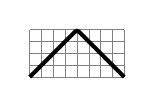
\begin{tikzpicture}[scale=0.15]  \draw[gray,very thin] (0, 0) grid (8, 4);  \draw[rounded corners=1, color=black, line width=1.5] (0, 0) -- (1, 1) -- (2, 2) -- (3, 3) -- (4, 4) -- (5, 3) -- (6, 2) -- (7, 1) -- (8, 0);\end{tikzpicture}$}}$};
  \node (node_12) at (1048.0bp,367.0bp) [draw,draw=none] {$\vcenter{\hbox{$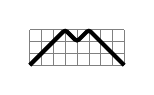
\begin{tikzpicture}[scale=0.15]  \draw[gray,very thin] (0, 0) grid (8, 3);  \draw[rounded corners=1, color=black, line width=1.5] (0, 0) -- (1, 1) -- (2, 2) -- (3, 3) -- (4, 2) -- (5, 3) -- (6, 2) -- (7, 1) -- (8, 0);\end{tikzpicture}$}}$};
  \node (node_1) at (623.0bp,107.0bp) [draw,draw=none] {$\vcenter{\hbox{$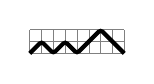
\begin{tikzpicture}[scale=0.15]  \draw[gray,very thin] (0, 0) grid (8, 2);  \draw[rounded corners=1, color=black, line width=1.5] (0, 0) -- (1, 1) -- (2, 0) -- (3, 1) -- (4, 0) -- (5, 1) -- (6, 2) -- (7, 1) -- (8, 0);\end{tikzpicture}$}}$};
  \node (node_10) at (876.0bp,223.0bp) [draw,draw=none] {$\vcenter{\hbox{$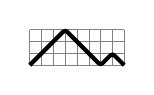
\begin{tikzpicture}[scale=0.15]  \draw[gray,very thin] (0, 0) grid (8, 3);  \draw[rounded corners=1, color=black, line width=1.5] (0, 0) -- (1, 1) -- (2, 2) -- (3, 3) -- (4, 2) -- (5, 1) -- (6, 0) -- (7, 1) -- (8, 0);\end{tikzpicture}$}}$};
  \node (node_11) at (469.0bp,511.0bp) [draw,draw=none] {$\vcenter{\hbox{$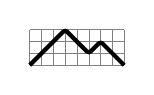
\begin{tikzpicture}[scale=0.15]  \draw[gray,very thin] (0, 0) grid (8, 3);  \draw[rounded corners=1, color=black, line width=1.5] (0, 0) -- (1, 1) -- (2, 2) -- (3, 3) -- (4, 2) -- (5, 1) -- (6, 2) -- (7, 1) -- (8, 0);\end{tikzpicture}$}}$};
  \node (node_0) at (623.0bp,19.0bp) [draw,draw=none] {$\vcenter{\hbox{$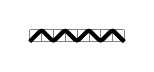
\begin{tikzpicture}[scale=0.15]  \draw[gray,very thin] (0, 0) grid (8, 1);  \draw[rounded corners=1, color=black, line width=1.5] (0, 0) -- (1, 1) -- (2, 0) -- (3, 1) -- (4, 0) -- (5, 1) -- (6, 0) -- (7, 1) -- (8, 0);\end{tikzpicture}$}}$};
  \draw [red,->] (node_1) ..controls (623.0bp,147.89bp) and (623.0bp,156.89bp)  .. (node_4);
  \draw [blue,->,dashed] (node_5) ..controls (267.78bp,154.06bp) and (229.62bp,171.25bp)  .. (node_7);
  \draw [blue,->,dashed] (node_2) ..controls (978.22bp,154.06bp) and (1016.4bp,171.25bp)  .. (node_3);
  \draw [red,->] (node_0) ..controls (703.03bp,47.204bp) and (739.52bp,59.607bp)  .. (node_2);
  \draw [red,->] (node_3) ..controls (1101.7bp,271.81bp) and (1090.1bp,292.17bp)  .. (node_12);
  \draw [red,->] (node_4) ..controls (623.0bp,278.31bp) and (623.0bp,287.03bp)  .. (node_13);
  \draw [red,->] (node_2) ..controls (876.0bp,147.89bp) and (876.0bp,156.89bp)  .. (node_10);
  \draw [blue,->,dashed] (node_10) ..controls (839.16bp,316.73bp) and (802.66bp,387.26bp)  .. (749.0bp,428.0bp) .. controls (704.94bp,461.45bp) and (647.52bp,481.29bp)  .. (node_11);
  \draw [red,->] (node_8) ..controls (200.14bp,409.12bp) and (222.33bp,419.35bp)  .. (243.0bp,428.0bp) .. controls (274.8bp,441.31bp) and (309.61bp,454.56bp)  .. (node_11);
  \draw [red,->] (node_0) ..controls (542.97bp,47.204bp) and (506.48bp,59.607bp)  .. (node_5);
  \draw [red,->] (node_5) ..controls (490.21bp,138.84bp) and (493.12bp,139.43bp)  .. (496.0bp,140.0bp) .. controls (604.27bp,161.39bp) and (636.96bp,149.25bp)  .. (node_10);
  \draw [blue,->,dashed] (node_10) ..controls (948.6bp,283.94bp) and (967.11bp,299.22bp)  .. (node_12);
  \draw [red,->] (node_6) ..controls (449.99bp,268.9bp) and (478.72bp,285.02bp)  .. (node_13);
  \draw [blue,->,dashed] (node_7) ..controls (117.0bp,275.69bp) and (117.0bp,302.1bp)  .. (node_8);
  \draw [red,->] (node_10) ..controls (776.3bp,279.96bp) and (757.43bp,290.55bp)  .. (node_13);
  \draw [red,->] (node_7) ..controls (204.15bp,272.91bp) and (243.42bp,294.95bp)  .. (node_9);
  \draw [red,->] (node_1) ..controls (520.78bp,154.06bp) and (482.62bp,171.25bp)  .. (node_6);
  \draw [blue,->,dashed] (node_6) ..controls (370.0bp,271.44bp) and (370.0bp,291.25bp)  .. (node_9);
  \draw [red,->] (node_0) ..controls (623.0bp,45.551bp) and (623.0bp,54.96bp)  .. (node_1);
  \draw [red,->] (node_5) ..controls (370.0bp,152.23bp) and (370.0bp,166.73bp)  .. (node_6);
  \draw [red,->] (node_2) ..controls (783.82bp,149.54bp) and (758.9bp,160.76bp)  .. (node_4);
%
\end{tikzpicture}
  \caption{Hasse diagram of the poset $(\Dyck_4, \leq)$. Edge colors will be explained and used in Section 10.1.}
  \label{fig_dyck4}
\end{figure}

